%%%%%%%%%%%%%%%%%%%%
% Typeset twice to get positioning right.
%%%%%%%%%%%%%%%%%%%%

\RequirePackage{luatex85}
\documentclass[letterpaper]{article}
\thispagestyle{empty}
\usepackage{tikz}
%\usetikzlibrary{patterns}

\def\ylist{{1.918, {sqrt(0.5^2+1.918^2)}, 1, 1, {1.5*pi/4}, 0.5, 1, 0.5, 1.918}}
\newcommand\diagram{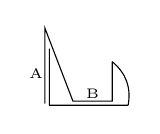
\begin{tikzpicture}[scale=0.5]
	\draw (0,0)
	-- node[pos=0.4, left, inner sep=0.2mm]{\tiny A} ++(up:\ylist[0])
	--++(-69:\ylist[1])
	-- node[above, inner sep=0.2mm]{\tiny B} ++(right:\ylist[2])
	--++(up:\ylist[3]) coordinate (temp)
	(temp) edge[-, bend left] ++(-70:\ylist[4]) ++(-70:\ylist[4])
	--++(left:\ylist[5]+\ylist[6]+\ylist[7])
	--++(up:\ylist[8]*0.75cm);
	\end{tikzpicture}}

\begin{document}
\sf

\begin{tikzpicture}[remember picture, overlay]
\draw (current page.north west) coordinate (0);
\foreach \n in {0,...,8}{
	\pgfmathtruncatemacro\nplusone{\n+1}
	\draw (\n) ++(down:\ylist[\n]*1in) coordinate (\nplusone);
	}
\foreach \n in {0, 2, 6, 8} 
	\fill[black!5!] (\n) -- ++(down:\ylist[\n]*1in) -- ++(right:8.5in) -- ++(up:\ylist[\n]*1in) -- (\n);
\foreach \n in {1, 3, 4, 5, 7} 
	\fill[white] (\n) -- ++(down:\ylist[\n]*1in) -- ++(right:8.5in) -- ++(up:\ylist[\n]*1in) -- (\n);
\foreach \n in {1, 2, 3, 4, 5, 8} 
	\draw (\n) edge[dashed, -] node[pos=0.1] {fold} node[pos=0.9] {fold} ++(right:8.5in);
\foreach \n in {6, 7} 
	\draw (\n) edge[-] ++(right:8.5in);
\foreach \n/\i/\j in {0/A/staple, 1/\diagram/{}, 2/B/staple, 6/B/staple, 8/A/staple}
	\draw (\n) ++(down:1/2*\ylist[\n]*1in)
		++(right:0.1*8.5in) node {\j}
		++(right:0.4*8.5in) node {\scalebox{4}{\i}}
		++(right:0.4*8.5in) node {\j}
		;
\end{tikzpicture}
\end{document}